        \item [2]

          \begin{itemize}
            \item
              After reducing to a triangle system we have:

              \sysdelim..
              \systeme{
                2x + 3y = 1,
                -6y = 6
              }

              So $y = -1$, back-substituting and solving for $x$ we get

              $2x + 3(-1) = 1 \implies 2x - 3 = 1 \implies 2x = 4 \implies x = 2$.

              So we have $x = 2, y = -1$.
            \item
              We verify that

              \[
                2 \begin{bmatrix}2 \\ 10\end{bmatrix} + (-1) \begin{bmatrix}3 \\ 9\end{bmatrix}
                = \begin{bmatrix}4 \\ 20\end{bmatrix} + \begin{bmatrix}-3 \\ -9\end{bmatrix}
                = \begin{bmatrix}1 \\ 11\end{bmatrix}
              \]
            \item
              If the right hand side changed to $\begin{bmatrix}4 \\ 44\end{bmatrix} = 4\begin{bmatrix}1 \\ 11\end{bmatrix}$,
              then the $x$ and $y$ values increase accordingly.

              That is $x = 4(2) = 8, y = 4(-1) = -4$
          \end{itemize}

        \item [7]
          \begin{enumerate}
            \item
              If $a = 2$, then elimination breaks down permanently.
              As we will end up in an inconsistent system.
            \item
              If $a = 0$, then elimination breaks down temporarily
              until the first equation is swapped for the second.
          \end{enumerate}

          We can solve by elimination if we swap the equations

          \sysdelim.\}
          \systeme{
            4x + 6y = 6,
            3y = -3
          }
          $\implies$
          \systeme{
            4x + 6y = 6,
            y = -1
          }
          $\implies$
          \systeme{
            4x = 12,
            y = -1
          }
          $\implies$
          \systeme{
            x = 3,
            y = -1
          }

          So, $x = 3, y = -1$.
        \item [9]

          \begin{itemize}
            \item These two equations have a solution only when $2b_1 = b_2$.
            \item There are infinitely many solutions.
            \item
              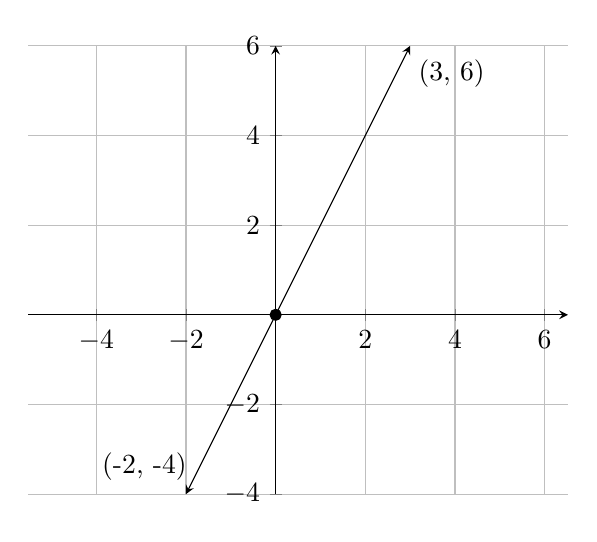
\begin{tikzpicture}
                \begin{axis}[axis equal, axis x line=middle, axis y line=middle, grid=major]
                  \addplot[-stealth]
                    coordinates { (0, 0) (3, 6) }
                    [xshift=15pt, yshift=-10pt]
                    node[pos=1] { (3, 6) }
                  ;
                  \addplot[-stealth]
                    coordinates { (0, 0) (-2, -4) }
                    [xshift=-15pt, yshift=10pt]
                    node[pos=1] { (-2, -4) }
                  ;
                  \addplot[only marks, mark=*] coordinates { (0, 0) };
                \end{axis}
              \end{tikzpicture}
          \end{itemize}
        \item [10]

          \sysdelim.\}
          \systeme{ 2x + 3y + z  = 8
                  , 4x + 7y + 5z = 20
                  ,    - 2y + 2z = 0
                  }
          $\implies$
          \systeme{ 2x + 3y + z  = 8
                  ,       y + 3z = 4
                  ,    - 2y + 2z = 0
                  }
          $\implies$
          \systeme{ 2x + 3y + z  = 8
                  ,       y + 3z = 4
                  ,         + 8z = 8
                  }

          The pivots are:

          \systeme{ \circled{2}x + 3y           + z            = 8
                  ,              + \circled{1}y + 3z           = 4
                  ,                             + \circled{8}z = 8
                  }

          We can solve by back substitution.

          \begin{itemize}
            \item $z = 1$
            \item $y + 3(1) = 4 \implies y + 3 = 4 \implies y = 1$
            \item $2x + 3(1) + 1 = 8 \implies 2x + 3 + 1 = 8 \implies 2x = 4 \implies x = 2$
          \end{itemize}

          So we have $x = 2, y = 1, z = 1$

        \item [12]
          \begin{itemize}
            \item

              If $d = 10$, then row 2 will need to be exchanged with row 3.
              As after one step the system will be:

              \sysdelim..
              \systeme{ 2x + 5y + z = 0
                      ,         - z = 2
                      ,       y - z = 3
                      }

            \item

              If $d = 11$, then the system is singular.
              As after one step the system will be:

              \systeme{ 2x + 5y + z = 0
                      ,       y - z = 2
                      ,       y - z = 3
                      }

              And this system cannot have a third pivot.
          \end{itemize}

        \item [13]

          \begin{itemize}
            \item

              If $b = 2$, then row 2 will need to be exchanged with row 3.
              As after one step the system will be:

              \sysdelim..
              \systeme{ x + 2y = 0
                      , -z = 0
                      , y + z = 0
                      }
            \item

              If $b = -1$, then the system is singular.
              As after one step the system will be:

              \sysdelim..
              \systeme{ x + 2y = 0
                      , -y -z = 0
                      , y + z = 0
                      }

              And this system cannot have a third pivot.
          \end{itemize}

        \item [24]
          \sysdelim.\}
          \systeme{ 2u - v = 0
                  , -u + 2v - w = 0
                  , -v + 2w - z = 0
                  , -w + 2z = 5
                  }
          $\implies$
          \systeme{ -u + 2v - w = 0
                  , 2u - v = 0
                  , -v + 2w - z = 0
                  , -w + 2z = 5
                  }
          $\implies$

          \systeme{ -u + 2v - w = 0
                  , 2u - v = 0
                  , -v + 2w - z = 0
                  , -w + 2z = 5
                  }
          $\implies$
          \systeme{ -u + 2v - w = 0
                  , 3v - 2w = 0
                  , -v + 2w - z = 0
                  , -w + 2z = 5
                  }
          $\implies$

          \systeme{ -u + 2v - w = 0
                  , -v + 2w - z = 0
                  , 3v - 2w = 0
                  , -w + 2z = 5
                  }
          $\implies$
          \systeme{ -u + 2v - w = 0
                  , -v + 2w - z = 0
                  , 4w - 3z = 0
                  , -w + 2z = 5
                  }
          $\implies$

          \systeme{ -u + 2v - w = 0
                  , -v + 2w - z = 0
                  , -w + 2z = 5
                  , 4w - 3z = 0
                  }
          $\implies$
          \systeme{ -u + 2v - w = 0
                  , -v + 2w - z = 0
                  , -w + 2z = 5
                  , 5z = 20
                  }

          Back-substituting we get:

          \begin{itemize}
            \item $z = 4$
            \item $-w + 2(4) = 5     \implies -w + 8     = 5 \implies w = 3$
            \item $-v + 2(3) - 4 = 0 \implies -v + 6 - 4 = 0 \implies v = 2$
            \item $-u + 2(2) - 3 = 0 \implies -u + 4 - 3 = 0 \implies u = 1$
          \end{itemize}

          So we have $u = 1, v = 2, w = 3, z = 4$,

          and pivots:
          \systeme{ \circled{-1}u + 2v - w = 0
                  , + \circled{-1}v + 2w - z = 0
                  , + \circled{-1}w + 2z = 5
                  , + \circled{5}z = 20
                  }
